% Difference table of x^2 at 0,1,2,3,4. Left edge 0,1,2; second differences constant.
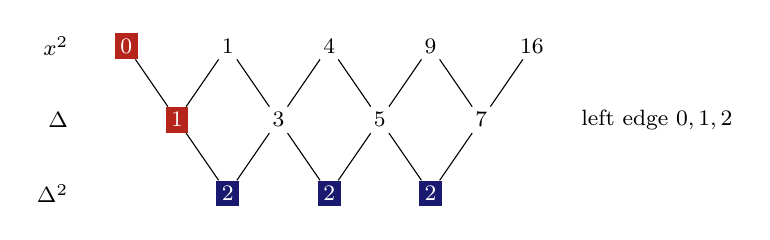
\begin{tikzpicture}[x=1.12cm,y=0.78cm,every node/.style={font=\footnotesize}]
  \node[anchor=east] at (-0.55,0) {$x^2$};
  \node[fill=BrickRed,text=white,inner sep=2pt] (a0) at (0,0) {$0$};
  \node[inner sep=2pt] (a1) at (1.15,0) {$1$};
  \node[inner sep=2pt] (a2) at (2.30,0) {$4$};
  \node[inner sep=2pt] (a3) at (3.45,0) {$9$};
  \node[inner sep=2pt] (a4) at (4.60,0) {$16$};
  \node[anchor=east] at (-0.55,-1.2) {$\Delta$};
  \node[fill=BrickRed,text=white,inner sep=2pt] (b0) at (0.575,-1.2) {$1$};
  \node[inner sep=2pt] (b1) at (1.725,-1.2) {$3$};
  \node[inner sep=2pt] (b2) at (2.875,-1.2) {$5$};
  \node[inner sep=2pt] (b3) at (4.025,-1.2) {$7$};
  \node[anchor=east] at (-0.55,-2.4) {$\Delta^2$};
  \node[fill=MidnightBlue,text=white,inner sep=2pt] (c0) at (1.15,-2.4) {$2$};
  \node[fill=MidnightBlue,text=white,inner sep=2pt] (c1) at (2.30,-2.4) {$2$};
  \node[fill=MidnightBlue,text=white,inner sep=2pt] (c2) at (3.45,-2.4) {$2$};
  \draw[black] (a0)--(b0)--(a1)--(b1)--(a2)--(b2)--(a3)--(b3)--(a4);
  \draw[black] (b0)--(c0)--(b1)--(c1)--(b2)--(c2)--(b3);
  \node[anchor=west] at (5.05,-1.2) {left edge $0,1,2$};
\end{tikzpicture}
